\chapter{Exponents and Radicals}
%%%%%%%%%%%%%%% SECTION HEADER %%%%%%%%%%%%%%%%
\rhead{3}
\lhead{Exponents and Radicals}
%%%%%%%%%%%%%%%%%%% START %%%$%%%%%%%%%%%%%%%%%
\section{Exponent expressions}
An exponent (also called power or degree) tells us how many times a number will be 
multiplied by itself. For example, consider $x^5$. The exponent is 5 and $x$ is 
called the base. This means that the variable $x$ will be multiplied by itself 5 
times. You can also think of this as $x$ to the fifth power.
\begin{figure}[ht]
\begin{center}
	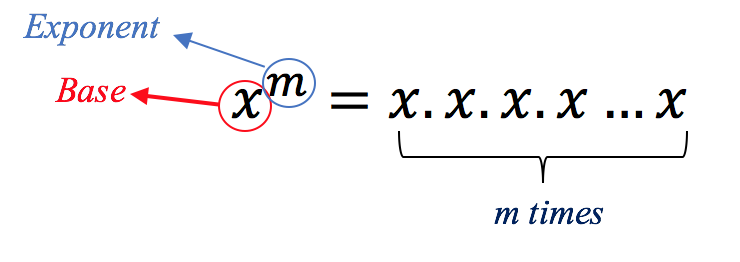
\includegraphics[width=8cm]{pics/exponent.png}
\end{center}
\end{figure}
\vspace{-1.3cm}
\subsection{Exponent Rules}
All of the exponent rules are summarized in the Table 1. Practice plays an important
role in learning exponent rules. Even if you forgot a particular rule, you can
prove it by your self using the definition of exponents.\\
For instance, let's consider $x^3\cdot x^5$. Here $x^3$ means that we should multiply $x$
by itself 3 times. Same thing for $x^5$: multiply the $x$ by itself 5 times.
\begin{align*}
	x^3\cdot x^5&=(x\cdot x\cdot x)(x\cdot x \cdot x \cdot x \cdot x) \\
				& = 	x\cdot x\cdot x\cdot x\cdot x \cdot x \cdot x \cdot x
\end{align*}
Since $x$ is multiplied by itself 8 times, we can write our final answer like this
\begin{align*}
	x^3\cdot x^5&= x^8
\end{align*}
As you can see, the summation of the exponents is $3+5=8$. So that's how we get our final solution when you multiply two numbers with the same bases-just need to add their exponents. Same thing if we have division. For example, $\displaystyle \frac{y^3}{y^2}$ is equal to
\begin{align*}
    \frac{y^3}{y^2} &= \frac{\bcancel{y}\cdot \bcancel{y}\cdot y}{\bcancel{y}\cdot \bcancel{y}}  \\
                    & = y
\end{align*}
\newpage
The same procedure can be used to prove for the following rules.
\begin{table}[h]
\begin{center}
    \caption{Exponent Rules}
	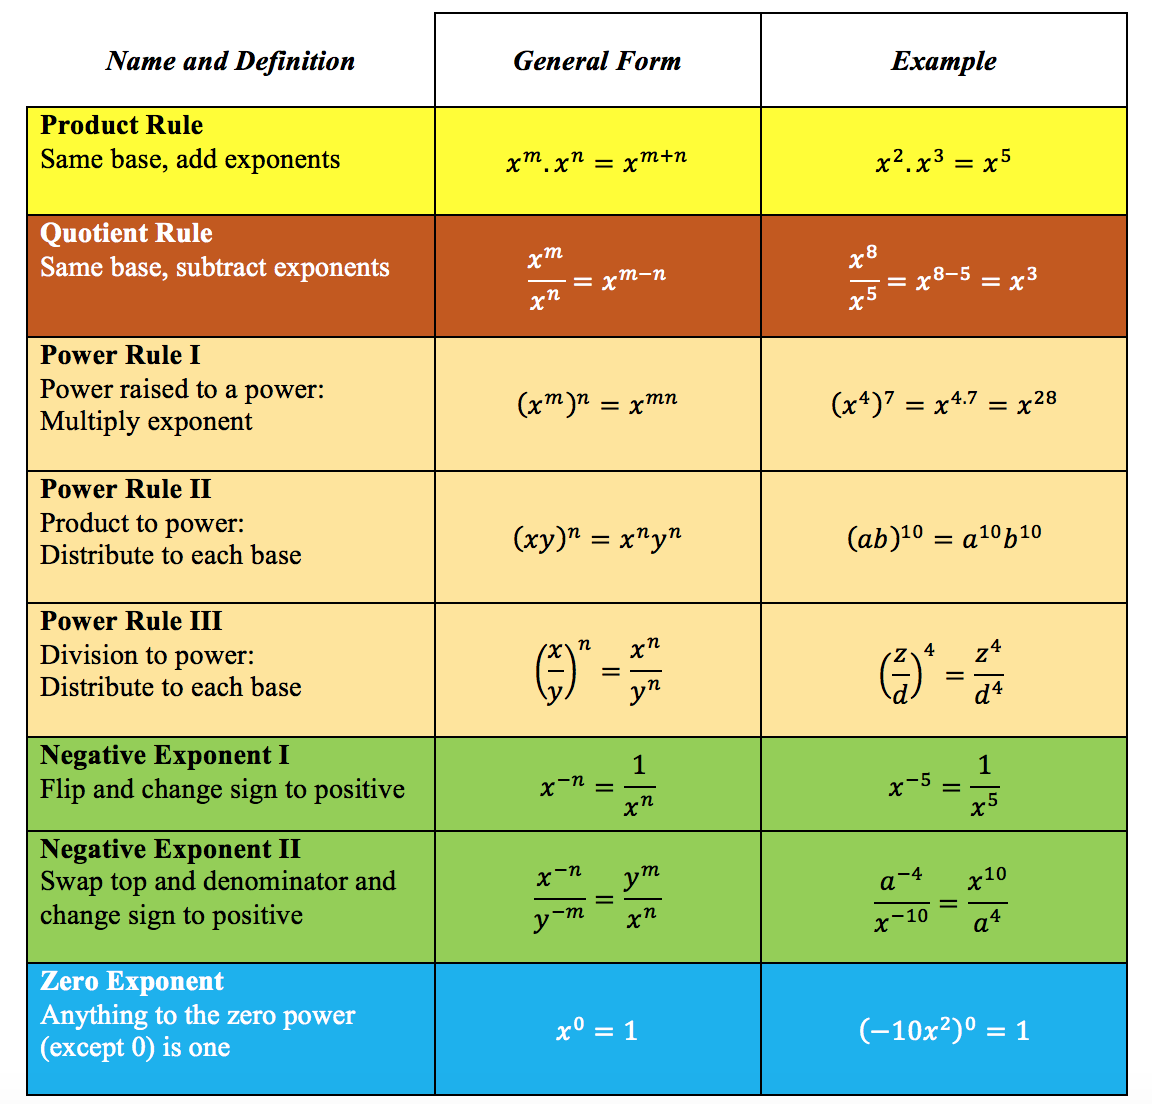
\includegraphics[width=\linewidth]{pics/exponent_rules.png}
	\label{tbl:exp_rules}
\end{center}
\end{table}
\section{Radical expressions}
While square roots are the most common type of radical we work with, we can take 
higher roots of numbers as well: cube roots, fourth roots, fifth roots, etc. The 
$n$th root of a number is a value that when multiplied by itself $n$ times, you will 
get the original number. 
		\begin{equation}
					\sqrt[n]{a} = b \Longleftrightarrow a = b^n	
		\end{equation}
The symbol $\sqrt{\quad}$ is called radical, and the small letter $n$ inside the 
radical is called the index. It tells us which root we are taking, or which power we
are “un-doing”.
		\begin{figure}[ht]
				
\includegraphics[width=6cm]{pics/radical.png}
				\centering
		\end{figure}
\subsection{Square and higher-root}
Remember the square root of a number is always positive.For square roots the index 
is 2. As this is the most common root, the two is not usually written.
\begin{align*}
			\sqrt{4} &=2		&&\text{because $2^2$=4}\\
			\sqrt[4]{81} &=3 	&&\text{because $3^4$=81}\\
			\sqrt[5]{16807} &=7		&&\text{because $7^5$=16807}\\
			\sqrt{-125} &=\text{\xmark} &&\text{Not defined in real numbers!!}\\
			\sqrt[3]{-64} &=-4 &&\text{because $(-4)^3$=-64}\\
			\sqrt[7]{-128} &=-2 &&\text{because $(-2)^7$=-128}
\end{align*}
We must be careful of a few things as we work with higher roots. 
\begin{enumerate}
\item It is important not to forget to check the index on the root. $\sqrt{81}=9$ 	
		but $\sqrt[4]{81}=3$. This is because $9^2 = 81$ and $3^4 = 81$. 
\item Another thing to watch out for is negative numbers under roots. We can take an 
		odd root of a negative number, because a negative number
		raised to an odd power is still negative. However, we cannot take an even
		root of a negative number. In this case, we will say is undefined. 
\end{enumerate}		
\begin{nt}
Later, we will discuss how to work with roots of negative, but for now 
we will simply say they are undefined.
\end{nt}
\begin{tcolorbox}[title=Radical in real realm, fonttitle=\bfseries,
                 colframe=blue!70!red,
                 colback =white]
	\begin{itemize}
		\item If index, $n$, is an odd number such as 3, 5, 7, 9, \ldots then
				\begin{align*}
				\sqrt[n]{\circled{+}} &= \circled{+} \,\,\checkmark &&\\[.2cm]
				\sqrt[n]{\circled{$-$}} &= \circled{$-$} \,\,\checkmark &&
				\end{align*}
		\item If index, $n$, is an even number such as 2, 4, 6, 8,\ldots then
				\begin{align*}
					\sqrt[n]{\circled{+}} &= \circled{+} \,\,\checkmark \hspace{2.6cm}\\
					\sqrt[n]{\circled{$-$}} &=\,\, \text{Not defined} \,\,\text{\xmark}
				\end{align*}
	\end{itemize}
\end{tcolorbox}
% ========== EXAMPLE 1
\begin{exa}
If possible, find the roots. If there is no real number root, say so.

\vspace{0.3cm}
a) $\sqrt[3]{216}$\qquad b)$\sqrt[5]{-32}$\qquad  c)$\sqrt[4]{-81}$
\end{exa}
\vspace{0.5cm}
a) The index is an odd number, we have an answer $\sqrt[3]{216}=6$.

\vspace{0.5cm}
b) Although the radicand is a negative number, the index is an odd number, so we still have an answer $\sqrt[5]{-32}=-2$.
\vspace{0.5cm}


c) The index is an even number, 4. Therefore, when the radicand is negative we won't have any real solution. $\sqrt[4]{-81}=$ not defined \xmark. The answer to this radical is actually an imaginary number which we learn how to deal with them later.
% ========= SUBSECTION
\subsection{Exponential Notation}
We can write the $n$th root in two different notations: One in radical form, which
we are already familiar with it; Or using the exponential form. The latter form,
is very useful especially when we want to simplify a root or logarithms.
\begin{tcolorbox}[title=Exponential Notation, fonttitle=\bfseries,
                 colframe=blue!70!red,
                 colback =white]
If $n$ is an integer greater than one and $x$ is an integer, then the $n$th root of $x$ can be expressed as 
						\begin{equation}
 								\sqrt[n]{x}=x^{1/n} \label{exp_notation}
 						\end{equation}	
\end{tcolorbox}
We can easily prove that $\sqrt[n]{x^m}$ is equal to $x^{m/n}$. We begin with the exponential notation form \eqref{exp_notation}:
\begin{align*}
		\sqrt[n]{x} &= x^{1/n} 		&&\text{Raise both sides to the power of $m$}\\
		\left(\sqrt[n]{x}\right)^{m} &= \left(x^{1/n}\right)^m &&\text{Use power rule I}\\
		\left(\sqrt[n]{x}\right)^{m} &= x^{m/n} &&\text{(i)}\\
\end{align*}
The left-hand side means to multiply $\sqrt[n]{x}$, $m$ times so
	\begin{align*}
			\left(\sqrt[n]{x}\right)^{m} &= \sqrt[n]{x}\cdot \sqrt[n]{x}\ldots\sqrt[n]{x} &&\\
		\left(\sqrt[n]{x}\right)^{m} &= \sqrt[n]{x^m} &&\text{(ii)}
	\end{align*}
Comparing (i) and (ii), we will get
\begin{equation*}
				\sqrt[n]{x^m} = x^{m/n}
\end{equation*}
According to this formula when $m=n$, we will get $\sqrt[n]{x^n}=x^{n/n}=x$. In other words, raising the $\sqrt[n]{x}$ to the power of $n$ yields to
$n$. This works very well when the index is an odd number.Examples are
\begin{align*}
			\sqrt[3]{10^3} &= 3\\
			\sqrt[5]{(-4)^5} &= -4
\end{align*}
However, when the index is an even number, we know we the answer of a root should
be a positive number. For example, $\sqrt[2]{(-3)^2}$ is equal to 3 not -3. To solve this problem,  we need to use absolute value.

\begin{tcolorbox}[title=Summary,fonttitle=\bfseries,                               colframe=blue!70!red,
                 colback =white]
	\begin{equation}
	        	\sqrt[n]{x^m} = x^{m/n} \label{exp_notationII}
	\end{equation}
	For all real $x$, 
	\begin{align}
		\sqrt[n]{x^n}&=|x|\ \ \text{, if $n$ is an even number.} \label{even}\\
		\sqrt[n]{x^n}&=x \ \ \ \ \!\text{, if $n$ is an odd number.}\label{odd}
	\end{align} 
\end{tcolorbox}
%========= EXAMPLE
\begin{exa}
Change to rational exponents and simplify.
\begin{enumerate}[\bfseries a.]
    \item $\sqrt[3]{x^3}$ 
    \item $\sqrt[4]{w^4}$
    \item $\sqrt[3]{125x^3y^6}$
\end{enumerate}
\end{exa}
a.
	\begin{align*}
			\sqrt[3]{x^3}&  &&\text{Use \eqref{odd}}\\
			x&		        &&\text{Our solution}\\
    \end{align*}
b.
    \begin{align*}
			\sqrt[4]{w^4}&  &&\text{Use \eqref{even}}\\
			|w|&	        &&\text{Our solution}\\
    \end{align*}
c.    
    \begin{align*}
			\sqrt[3]{125x^3y^6}& &&\text{Use \eqref{exp_notationII}}\\
			\left(125x^3y^6\right)^{1/3}&	&&\text{Use power rule II}\\[.2cm]
			125^{(1/3)}x^{(3)(1/3)}y^{(6)(1/3)}& &&\text{Simplify}\\
			5xy^2&	&&\text{Our solution}
	\end{align*}
